\documentclass[14pt,aspectratio=169,xcolor={usenames,dvipsnames}]{beamer}
\usetheme{Frankfurt}
\usepackage[utf8]{inputenc}
\usepackage[T1]{fontenc}
\usepackage{lmodern}
\usepackage[australian]{babel}
%\usepackage{amsfonts}
%\usepackage{csquotes}
\usepackage{tikz}
%\usepackage{multirow}
\usepackage{pgfplots}
%\usepackage{booktabs}
\usepackage{siunitx}
%\usepackage{algorithm2e}
\usepackage[super]{nth}
%\usepackage[hidelinks]{hyperref}

\pgfplotsset{compat=1.5}



\author{Sébastien Vaucher \and Benjamin Bediako}
\title{Tree-based Routing}
%\setbeamercovered{transparent} 
%\setbeamertemplate{navigation symbols}{} 
%\logo{}
%\institute{Université de Neuchâtel}
\date{14 December 2015}
\subject{Sensor Network \& Internet of Things}
\begin{document}

\begin{frame}[plain]
\titlepage
\begin{center}
Sensor Networks \& Internet of Things\\
University of Bern
\end{center}
\end{frame}

\begin{frame}{Contents}
\tableofcontents
\end{frame}



\section{The algorithm}

\subsection{Theoretical introduction}

\begin{frame}{Goal of the algorithm}

\begin{enumerate}
\item Establish a tree of nodes
\begin{itemize}
\item The \textbf{sink} is the root of the tree
\end{itemize}
\item Route sensor data towards the sink
\end{enumerate}
\end{frame}


\begin{frame}{Two phases}
\begin{enumerate}
\item Discovery phase
\begin{enumerate}
\item Regularly \textit{flood} discovery packets from the sink
\item Re-broadcast the packet at intermediate nodes
\item $\rightarrow$ Only if interesting packet
\item Choose parent according to strategy
\end{enumerate}
\item Send temperature data hop-by-hop
\begin{enumerate}
\item Each node sends to its parent
\item Recursively forward until sink is reached
\end{enumerate}
\end{enumerate}
\end{frame}

\subsection{Implementation}

\begin{frame}{Algorithm configuration}
\begin{enumerate}
\item 2 MAC protocols
\begin{itemize}
\item NullMAC
\item X-MAC
\end{itemize}
\item 2 parent choice strategies
\begin{itemize}
\item Lowest hop-count
\item Highest RSSI (best signal quality)
\end{itemize}
\end{enumerate}
\end{frame}


\section{Analysis}

\subsection{Methodology}

\begin{frame}{Producing data}
To produce data to analyze, we added some \textsf{printf}
\vspace{1cm}
\begin{block}{Sink}
Every \SI{30}{\second}, print the hop-count distribution of incoming packets
\end{block}
\begin{block}{Sensor nodes}
When setting a new parent, output its ID
\end{block}
\end{frame}


\begin{frame}{Parsing the generated data}
Custom Python script with embedded XML parser.\\
It generates:

\begin{enumerate}
\item All numerical statistics
\item A 3D representation of the links between nodes
\end{enumerate}
\end{frame}

\subsection{Results}

\begin{frame}
\begin{columns}
\column{0.6\textwidth}
\begin{figure}

    \begin{tikzpicture}[scale=0.097,y= {(0.281cm,0.281cm)}, z={(0cm,1cm)}, x={(1cm,0cm)}]]
    \node[anchor=south west,inner sep=0] at (0,0) {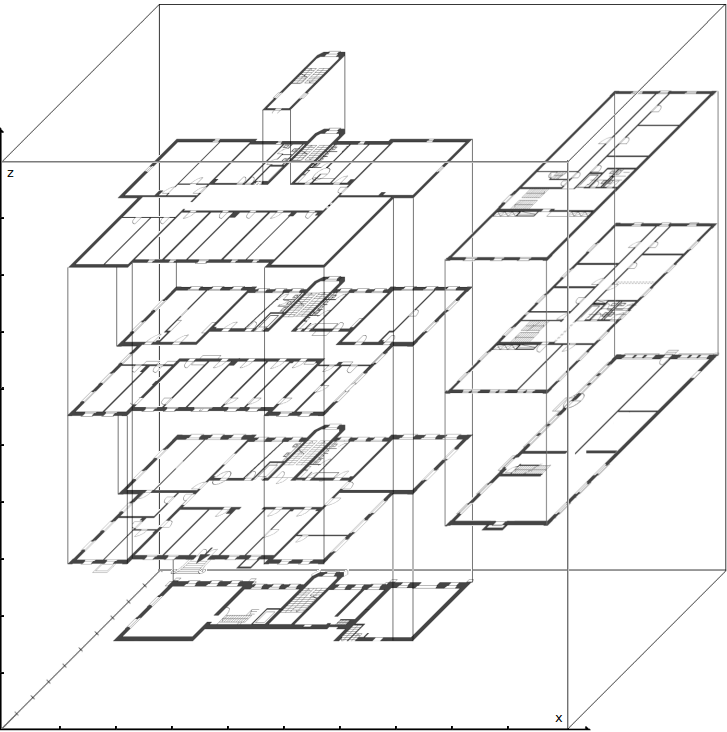
\includegraphics[width=\textwidth]{3D_image_iam_complete.png}};
    \draw [Maroon, thick, dash pattern= on 4mm off 4mm, dash phase=2mm, <-, >=latex] (45,25,52) to (52,30,80);
\draw [Maroon, thick, dash pattern= on 4mm off 4mm, dash phase=2mm, <-, >=latex] (45,25,52) to (45,98,22);
\draw [Maroon, thick, dash pattern= on 4mm off 4mm, dash phase=2mm, <-, >=latex] (45,98,22) to (80,10,80);
\draw [Maroon, thick, dash pattern= on 4mm off 4mm, dash phase=2mm, <-, >=latex] (80,10,80) to (90,100,85);
\draw [Maroon, thick, dash pattern= on 4mm off 4mm, dash phase=2mm, <-, >=latex] (45,25,52) to (53,33,52);
\draw [Maroon, thick, dash pattern= on 4mm off 4mm, dash phase=2mm, <-, >=latex] (45,25,52) to (37,55,52);
\draw [Maroon, thick, dash pattern= on 4mm off 4mm, dash phase=2mm, <-, >=latex] (37,55,52) to (3,75,22);
\draw [Maroon, thick, dash pattern= on 4mm off 4mm, dash phase=2mm, <-, >=latex] (37,55,52) to (20,35,52);
\draw [Maroon, thick, dash pattern= on 4mm off 4mm, dash phase=2mm, <-, >=latex] (45,25,52) to (37,15,80);
\draw [Maroon, thick, dash pattern= on 4mm off 4mm, dash phase=2mm, <-, >=latex] (45,25,52) to (48,65,22);
\draw [Maroon, thick, dash pattern= on 4mm off 4mm, dash phase=2mm, <-, >=latex] (48,65,22) to (90,10,80);
\draw [Maroon, thick, dash pattern= on 4mm off 4mm, dash phase=2mm, <-, >=latex] (48,65,22) to (16,30,22);
\draw [Maroon, thick, dash pattern= on 4mm off 4mm, dash phase=2mm, <-, >=latex] (45,25,52) to (47,85,80);
\draw [Maroon, thick, dash pattern= on 4mm off 4mm, dash phase=2mm, <-, >=latex] (45,25,52) to (45,35,22);
\draw [Maroon, thick, dash pattern= on 4mm off 4mm, dash phase=2mm, <-, >=latex] (45,25,52) to (53,53,80);
\draw [Maroon, thick, dash pattern= on 4mm off 4mm, dash phase=2mm, <-, >=latex] (53,53,80) to (5,60,80);
\draw [Maroon, thick, dash pattern= on 4mm off 4mm, dash phase=2mm, <-, >=latex] (45,25,52) to (19,80,52);
\draw [Maroon, thick, dash pattern= on 4mm off 4mm, dash phase=2mm, <-, >=latex] (19,80,52) to (78,78,57);
\draw [Maroon, thick, dash pattern= on 4mm off 4mm, dash phase=2mm, <-, >=latex] (78,78,57) to (90,100,80);
\draw [Maroon, thick, dash pattern= on 4mm off 4mm, dash phase=2mm, <-, >=latex] (19,80,52) to (18,55,0);
\draw [Maroon, thick, dash pattern= on 4mm off 4mm, dash phase=2mm, <-, >=latex] (19,80,52) to (78,63,57);
\draw [Maroon, thick, dash pattern= on 4mm off 4mm, dash phase=2mm, <-, >=latex] (78,63,57) to (80,75,80);
\draw [Maroon, thick, dash pattern= on 4mm off 4mm, dash phase=2mm, <-, >=latex] (78,63,57) to (93,78,57);
\draw [Maroon, thick, dash pattern= on 4mm off 4mm, dash phase=2mm, <-, >=latex] (45,25,52) to (38,40,22);
\draw [JungleGreen, thick, dash pattern= on 4mm off 4mm, dash phase=6mm, <-, >=latex] (45,25,52) to (38,40,22);
\draw [JungleGreen, thick, dash pattern= on 4mm off 4mm, dash phase=6mm, <-, >=latex] (38,40,22) to (16,30,22);
\draw [JungleGreen, thick, dash pattern= on 4mm off 4mm, dash phase=6mm, <-, >=latex] (16,30,22) to (16,55,22);
\draw [JungleGreen, thick, dash pattern= on 4mm off 4mm, dash phase=6mm, <-, >=latex] (45,25,52) to (37,15,80);
\draw [JungleGreen, thick, dash pattern= on 4mm off 4mm, dash phase=6mm, <-, >=latex] (45,25,52) to (35,20,52);
\draw [JungleGreen, thick, dash pattern= on 4mm off 4mm, dash phase=6mm, <-, >=latex] (45,25,52) to (48,65,22);
\draw [JungleGreen, thick, dash pattern= on 4mm off 4mm, dash phase=6mm, <-, >=latex] (45,25,52) to (45,90,52);
\draw [JungleGreen, thick, dash pattern= on 4mm off 4mm, dash phase=6mm, <-, >=latex] (45,90,52) to (85,33,57);
\draw [JungleGreen, thick, dash pattern= on 4mm off 4mm, dash phase=6mm, <-, >=latex] (85,33,57) to (92,33,57);
\draw [JungleGreen, thick, dash pattern= on 4mm off 4mm, dash phase=6mm, <-, >=latex] (85,33,57) to (78,78,57);
\draw [JungleGreen, thick, dash pattern= on 4mm off 4mm, dash phase=6mm, <-, >=latex] (78,78,57) to (90,100,80);
\draw [JungleGreen, thick, dash pattern= on 4mm off 4mm, dash phase=6mm, <-, >=latex] (45,25,52) to (53,53,80);
\draw [JungleGreen, thick, dash pattern= on 4mm off 4mm, dash phase=6mm, <-, >=latex] (53,53,80) to (80,10,80);
\draw [JungleGreen, thick, dash pattern= on 4mm off 4mm, dash phase=6mm, <-, >=latex] (80,10,80) to (90,100,85);
\draw [JungleGreen, thick, dash pattern= on 4mm off 4mm, dash phase=6mm, <-, >=latex] (45,25,52) to (20,39,80);
\draw [JungleGreen, thick, dash pattern= on 4mm off 4mm, dash phase=6mm, <-, >=latex] (20,39,80) to (20,35,52);
\draw [JungleGreen, thick, dash pattern= on 4mm off 4mm, dash phase=6mm, <-, >=latex] (45,25,52) to (45,98,22);
\draw [JungleGreen, thick, dash pattern= on 4mm off 4mm, dash phase=6mm, <-, >=latex] (45,98,22) to (89,10,57);
\draw [JungleGreen, thick, dash pattern= on 4mm off 4mm, dash phase=6mm, <-, >=latex] (45,98,22) to (78,63,57);
\draw [JungleGreen, thick, dash pattern= on 4mm off 4mm, dash phase=6mm, <-, >=latex] (78,63,57) to (80,75,80);
\draw [JungleGreen, thick, dash pattern= on 4mm off 4mm, dash phase=6mm, <-, >=latex] (78,63,57) to (80,100,80);
\draw [JungleGreen, thick, dash pattern= on 4mm off 4mm, dash phase=6mm, <-, >=latex] (45,25,52) to (37,55,52);
\draw [JungleGreen, thick, dash pattern= on 4mm off 4mm, dash phase=6mm, <-, >=latex] (37,55,52) to (3,75,22);
\draw [JungleGreen, thick, dash pattern= on 4mm off 4mm, dash phase=6mm, <-, >=latex] (45,25,52) to (52,30,80);
\draw [JungleGreen, thick, dash pattern= on 4mm off 4mm, dash phase=6mm, <-, >=latex] (52,30,80) to (5,60,80);
\draw [JungleGreen, thick, dash pattern= on 4mm off 4mm, dash phase=6mm, <-, >=latex] (45,25,52) to (19,80,52);
\draw [JungleGreen, thick, dash pattern= on 4mm off 4mm, dash phase=6mm, <-, >=latex] (19,80,52) to (18,55,0);
\node [blue, very thick] (1) at (45,25,52) {$\bullet$};\node [blue, very thick] (2) at (53,33,52) {$\bullet$};\node [blue, very thick] (3) at (20,15,80) {$\bullet$};\node [blue, very thick] (4) at (20,39,80) {$\bullet$};\node [blue, very thick] (5) at (47,85,80) {$\bullet$};\node [blue, very thick] (6) at (52,30,80) {$\bullet$};\node [blue, very thick] (7) at (10,70,80) {$\bullet$};\node [blue, very thick] (8) at (5,60,80) {$\bullet$};\node [blue, very thick] (9) at (55,80,52) {$\bullet$};\node [blue, very thick] (10) at (45,90,52) {$\bullet$};\node [blue, very thick] (11) at (35,20,52) {$\bullet$};\node [blue, very thick] (12) at (37,55,52) {$\bullet$};\node [blue, very thick] (13) at (40,45,80) {$\bullet$};\node [blue, very thick] (14) at (19,80,52) {$\bullet$};\node [blue, very thick] (15) at (16,55,22) {$\bullet$};\node [blue, very thick] (16) at (16,30,22) {$\bullet$};\node [blue, very thick] (17) at (6,55,0) {$\bullet$};\node [blue, very thick] (18) at (18,55,0) {$\bullet$};\node [blue, very thick] (19) at (38,40,22) {$\bullet$};\node [blue, very thick] (20) at (30,60,95) {$\bullet$};\node [blue, very thick] (21) at (48,65,22) {$\bullet$};\node [blue, very thick] (22) at (3,75,22) {$\bullet$};\node [blue, very thick] (23) at (20,35,52) {$\bullet$};\node [blue, very thick] (24) at (45,35,22) {$\bullet$};\node [blue, very thick] (25) at (45,98,22) {$\bullet$};\node [blue, very thick] (26) at (80,10,80) {$\bullet$};\node [blue, very thick] (27) at (90,10,80) {$\bullet$};\node [blue, very thick] (28) at (85,10,57) {$\bullet$};\node [blue, very thick] (29) at (78,63,57) {$\bullet$};\node [blue, very thick] (30) at (80,75,80) {$\bullet$};\node [blue, very thick] (31) at (80,100,80) {$\bullet$};\node [blue, very thick] (32) at (90,100,80) {$\bullet$};\node [blue, very thick] (33) at (89,10,57) {$\bullet$};\node [blue, very thick] (34) at (78,78,57) {$\bullet$};\node [blue, very thick] (35) at (93,78,57) {$\bullet$};\node [blue, very thick] (36) at (92,33,57) {$\bullet$};\node [blue, very thick] (37) at (85,33,57) {$\bullet$};\node [blue, very thick] (38) at (90,100,85) {$\bullet$};\node [blue, very thick] (39) at (53,53,80) {$\bullet$};\node [blue, very thick] (40) at (37,15,80) {$\bullet$};\end{tikzpicture}
\end{figure}
\column{0.4\textwidth}
\begin{itemize}
\item Ti\textit{k}Z picture generated by the Python script
\item MAC = X-MAC
\end{itemize}
\vspace{2.5cm}
\begin{block}{Legend}
\colorbox{Maroon}{\color{white}hop-count} \colorbox{JungleGreen}{RSSI}
\end{block}
\end{columns}
\end{frame}



\begin{frame}{Hop-counts distribution}
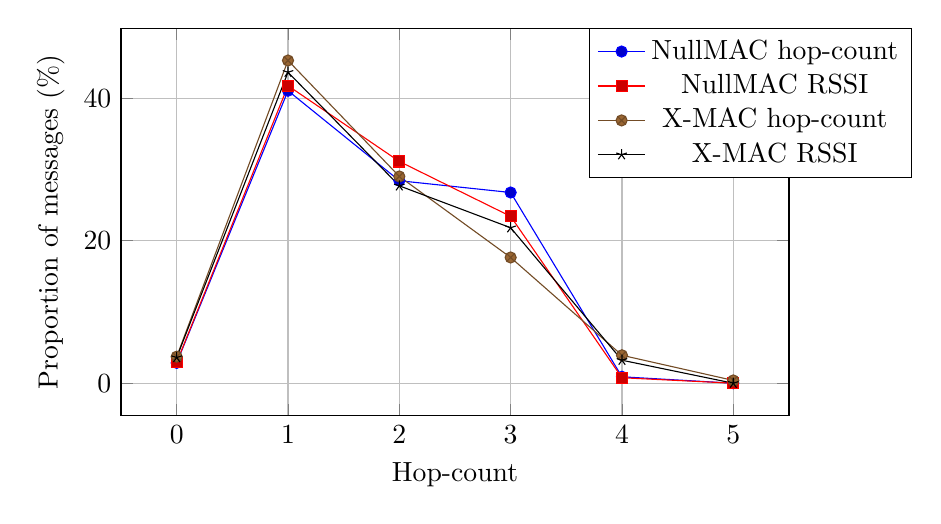
\begin{tikzpicture}[scale=1]
\begin{axis}[
	grid=major,
	height=6.5cm,
	width=0.83\textwidth,
	ylabel={Proportion of messages (\%)},
	xlabel={Hop-count},
	legend style={at={(0.7,1)}, anchor=north west,legend columns=1},
]
\addplot coordinates {(0, 2.857142857142857) (1, 41.05263157894737) (2, 28.421052631578947) (3, 26.766917293233083) (4, 0.9022556390977444) (5,0)};
\addplot coordinates {(0, 2.9275808936825885) (1, 41.756548536209553) (2, 31.124807395993837) (3, 23.420647149460708) (4, 0.7704160246533128) (5,0)};
\addplot coordinates {(0, 3.725490196078431) (1, 45.294117647058824) (2, 29.01960784313726) (3, 17.647058823529413) (4, 3.92156862745098) (5, 0.392156862745098)};
\addplot coordinates {(0, 3.6053130929791274) (1, 43.64326375711575) (2, 27.703984819734345) (3, 21.821631878557876) (4, 3.225806451612903) (5,0)};

\legend{NullMAC hop-count, NullMAC RSSI, X-MAC hop-count, X-MAC RSSI}
\end{axis}
\end{tikzpicture}
\end{frame}



\begin{frame}{Metrics}
\begin{columns}

\column{0.5\textwidth}
\textbf{Average hop-count}
\vspace{5mm}
\begin{tabular}{c|c|c|}
& Hop-count & RSSI \\
\hline
X-MAC & 2.72 & 2.61 \\
NullMAC & 2.77 & 2.73 \\
\end{tabular}

\column{0.5\textwidth}
\textbf{Average physical link length}
\vspace{5mm}
\begin{tabular}{c|c|c|}
& Hop-count & RSSI \\
\hline
X-MAC & 49.52 & 46.06 \\
\end{tabular}

\textbf{Percentage of connected nodes}
\begin{tabular}{c|c|c|}
& Hop-count & RSSI \\
\hline
X-MAC & \SI{72.5}{\percent} & \SI{67.5}{\percent} \\
\end{tabular}

\end{columns}
\end{frame}


\begin{frame}{Packet delivery rate}
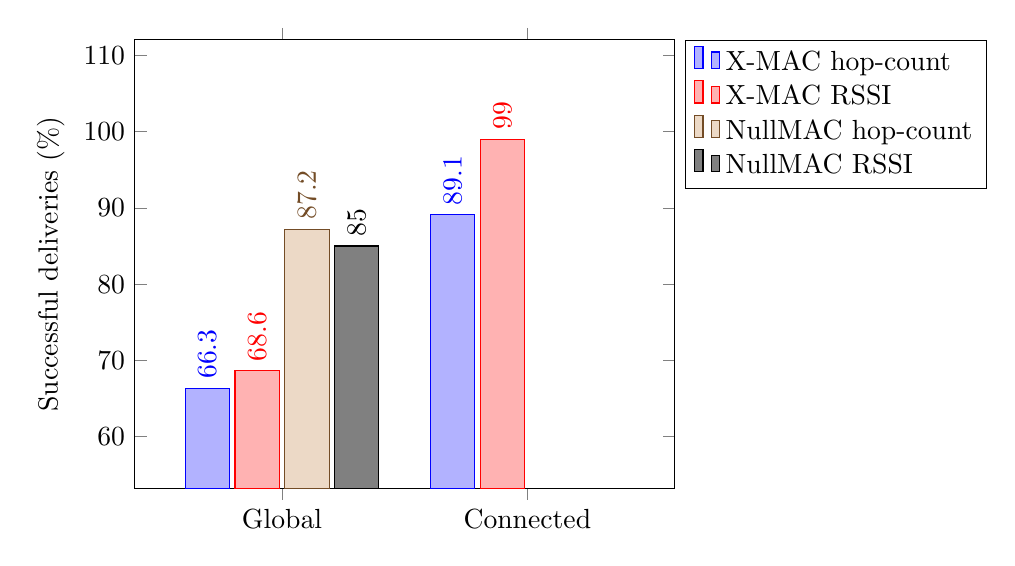
\begin{tikzpicture}[scale=1.0]
\begin{axis}[
	ybar,
	legend style={at={(1.02,1)}, anchor=north west,legend columns=1},
	legend cell align=left,
	symbolic x coords={Global,Connected},
	ylabel={Successful deliveries (\%)},
	enlarge x limits=0.6,
	enlarge y limits=0.4,
	nodes near coords,
	xtick=data,
	bar width={16},
	every node near coord/.append style={rotate=90, anchor=west}
]

\addplot coordinates { (Global,66.3) (Connected,89.1) };
\addplot coordinates { (Global,68.6) (Connected,99.0) };
\addplot coordinates { (Global,87.2) };
\addplot coordinates { (Global,85.0) };

\legend{X-MAC hop-count, X-MAC RSSI, NullMAC hop-count, NullMAC RSSI}
\end{axis}
\end{tikzpicture}
\end{frame}

\section{Conclusion}

\begin{frame}{Encountered problems}
\begin{enumerate}
\item On TARWIS using NullMAC, \textsf{printf} does not always arrive
\begin{itemize}
\item Impossible to parse child relations
\item Some statistics missing
\end{itemize}
\item Less than $\frac{3}{4}$ of the nodes managed to connect
\end{enumerate}
\end{frame}

\begin{frame}{Conclusion}
\begin{itemize}
\item Our implementation works
\item NullMAC (seems to) perform better
\item The RSSI strategy is the best
\item[]
\item Possible improvements
\begin{itemize}
\item Return channel
\item Implies sending ACKs to parent
\end{itemize}
\end{itemize}
\end{frame}

\end{document}